\section{Comparison with Alternative Approaches}
\label{sec:comparison}

The evaluation in \S\ref{sec:evaluation} establishes that \eps fires
on the prompts it is designed to catch and that its token-level
focus narrows the within-function review surface by $89\%$.
What it does not establish is whether \eps is the right signal
relative to alternatives that read the same raw logprob data, or to
alternatives that use the same underlying model via a different
protocol. This section provides that comparison. The organizing
point is simple: the function-level question --- ``which functions
need scrutiny?'' --- is answered roughly equally well by \eps, by
\papg~\cite{spiess2025calibration}, and (much worse) by multi-sample
methods. The token-level question --- ``where within the function?''
--- is answered only by \eps.

\subsection{Signal taxonomy}
\label{subsec:signal-taxonomy}

Three fundamentally different uncertainty signals are in play.
\textbf{Intra-generational token-level entropy} (\eps; AdaDec) reads
the top-$k$ distribution at each decoding step and preserves per-%
token scores. \textbf{Sequence-level aggregate probability} (\papg;
the Spiess et al.~\cite{spiess2025calibration} signal) averages log-%
probabilities over all generated tokens to produce a single scalar
per function. \textbf{Inter-generational behavioural diversity}
(multi-sample methods, UQLM~\cite{uqlm2024}) runs the model multiple
times at nonzero temperature and measures output-level agreement.

These are not three implementations of the same idea. The first two
happen to read the same raw logprob data at the same $1\times$ API
cost, but aggregate it differently: \eps localizes to a single
high-entropy token after syntactic filtering, while \papg smooths
over the entire sequence. The third requires multiple model calls
and measures a fundamentally different quantity: it cannot observe
internal distributions at all, only the outputs those distributions
produce.

\subsection{\papg: credit where due, and the distinguishing gap}
\label{subsec:papg-comp}

We compute \papg directly from the \texttt{mean\_logprob} fields in
the same calibration runs used to produce
Table~\ref{tab:calibration}: $\papg = \exp(\mathrm{mean\_logprob})$,
with higher values indicating higher confidence. For a fair
comparison, we choose the \papg decision threshold on each model so
that the resulting \textsc{low} false-positive rate matches \eps's
rate on that model; we then report the \textsc{high} detection rate
achieved at that operating point.

\begin{table}[h]
\centering
\small
\begin{tabular}{lrrrr}
\toprule
 & \multicolumn{2}{c}{\eps (\textsc{flagged+})} & \multicolumn{2}{c}{\papg (matched FP)} \\
\cmidrule(lr){2-3}\cmidrule(lr){4-5}
Model & \textsc{high} det. & \textsc{low} FP & \textsc{high} det. & \textsc{low} FP \\
\midrule
GPT-4o       & $85\%$ (17/20) & $50\%$ & $85\%$ (17/20) & $50\%$ \\
GPT-4o-mini  & $70\%$ (14/20) & $60\%$ & $75\%$ (15/20) & $10\%$ \\
GPT-4-turbo  & $70\%$ (14/20) & $60\%$ & $90\%$ (18/20) & $40\%$ \\
DeepSeek V3  & $85\%$ (17/20) & $70\%$ & $65\%$ (13/20) & $10\%$ \\
\bottomrule
\end{tabular}
\caption{\eps vs.\ \papg across four models at the function level.
\papg ties \eps on GPT-4o and outperforms \eps on GPT-4o-mini and
GPT-4-turbo on raw \textsc{high} detection; on DeepSeek V3, \eps is
higher ($85\%$ vs.\ $65\%$). At the same $1\times$ API cost, the raw
function-level detection picture favours neither signal uniformly.
\textsc{high} det.\ here is the flagging rate on \textsc{high}-category
prompts, not recall on true failures: when the model generates
correct code for a \textsc{high} prompt, \eps correctly produces
\textsc{complete} (low \eps), and those entries lower this rate
without representing missed failures.}
\label{tab:papg}
\end{table}

\paragraph{\papg's real strength, stated plainly.}
On three of four OpenAI models, \papg matches or beats \eps's
\textsc{high} detection rate at the same or lower \textsc{low} false-%
positive rate, using the same API call and the same logprobs. On
GPT-4-turbo it is $90\%$ vs.\ \eps's $70\%$ at a lower FP rate. This
is not a small finding, and we do not want to bury it. For a user
who only needs a function-level score and is working with the OpenAI
API, \papg is a strong, cheap, publicly-documented baseline.

\paragraph{Where \papg stops, and \eps continues.}
\papg produces one scalar per function. It cannot tell a reviewer
\emph{where in the function} the uncertainty lives. On the Stripe
example in Figure~\ref{fig:intra-inter}, \papg reports a single
number for the $98$-token function; \eps reports the same kind of
function-level score \emph{plus} an identification of the tokens
whose per-token entropy drove it. The reviewer does not need
to re-read the function --- they need to evaluate the method-%
selector decision (see Table~\ref{tab:token-focus}).

This is the distinguishing claim. It is not a higher rate; it is a
different kind of output. We ran the \papg baseline through the full
review loop to measure whether that attribution gap produces a
precision gap at the system level.

\paragraph{\papg through the review loop.}
We re-ran all six production and scenario result files with
\texttt{mean\_logprob} captured, swept \papg thresholds to find the
one whose API-entry recall best matches \eps's $93\%$, and ran the
identical review loop without providing token attribution to the reviewer.
The threshold sweep surfaces a structural constraint first: at every
threshold, \papg's maximum recall on API entries is $44\%$ ($76/174$).
Even at the most aggressive threshold, \texttt{mean\_logprob} stays
near zero across production completions --- the model is globally
confident, and averaging over the full token sequence absorbs the
localized uncertainty that \eps reads at the decision token.

At the matched threshold (\texttt{-mean\_logprob} $\ge 0.05$),
\papg flags $99$ entries. Through the review loop, end-to-end
precision is $50.5\%$ ($50/99$ confirmed true failures), compared
to \eps's $94\%$ on $200$ entries. All $50$ suspect entries were
confirmed by the consolidation pass ($0$ downgrades): the reviewer
correctly identified issues when it found them, but cleared $49$
genuine problems it could not localize to specific tokens.

\begin{table}[h]
\centering
\small
\begin{tabular}{lrrrr}
\toprule
Signal & Entries reviewed & API recall & End-to-end precision & True errors found \\
\midrule
\eps (cascaded)               & $200$ & $93\%$ ($162/174$) & $\mathbf{94\%}$ & ${\sim}188$ \\
\papg (${\ge}0.05$ threshold) & $\phantom{0}99$ & $44\%$ ($\phantom{0}76/174$) & $50.5\%$ & $\phantom{{\sim}0}50$ \\
\bottomrule
\end{tabular}
\caption{End-to-end comparison: \eps vs.\ \papg through the full review loop on the
same 228-entry production-plus-scenario set (three models). \papg's recall ceiling is
structural: \texttt{mean\_logprob} averages over all tokens including confident boilerplate,
absorbing localized API-decision uncertainty. The precision gap ($43.5$pp) reflects the
reviewer's inability to localize without token attribution; errors were confirmed when
found but $49$ genuine failures were cleared because the reviewer had no token target to
examine.}
\label{tab:pavg-endtoend}
\end{table}

The system-level conclusion differs from the signal-level one.
Token attribution is not a refinement on top of the filter; it is
the mechanism that enables $94\%$ end-to-end precision. Without it,
the same review loop achieves $50.5\%$.

\paragraph{\texttt{min\_logprob} as a sanity floor.}
The older single-token \texttt{min\_logprob} baseline
(Table~\ref{tab:logprob}) is complementary to both signals. It looks
at the lowest top-$1$ probability in the generation, which misses
near-tie tokens (e.g., $0.48/0.42$): the top-$1$ is still $0.48$
and the threshold does not fire. \eps sees near-uniform top-$k$
entropy on the same token and does.

\begin{table}[h]
\centering
\small
\begin{tabular}{lrr}
\toprule
Method & \textsc{high} det.\ @ $30\%$ \textsc{low} FP
       & \textsc{high} det.\ @ $50\%$ \textsc{low} FP \\
\midrule
\texttt{min\_logprob}       & $45$--$55\%$ & $55$--$65\%$ \\
\eps (max, AST-filtered)    & $\mathbf{70\%}$ & $\mathbf{85\%}$ \\
\bottomrule
\end{tabular}
\caption{Matched \textsc{low} FP budgets across four models, single
top-$1$ probability baseline. Gap is at near-tie tokens:
\texttt{min\_logprob} sees $0.48$ and does not fire; \eps sees
near-uniform top-$k$ entropy and does.}
\label{tab:logprob}
\end{table}

\subsection{Multi-sample: structural blindspot}
\label{subsec:multisample-comp}

Inter-generational methods measure disagreement across multiple
outputs of the same prompt. We ran each of the four models $N=5$
times at temperature $T=0.7$ on the full 30-prompt calibration
benchmark, and compute output diversity by extracting the API-choice
classification for each sample (e.g., \texttt{Charge} vs.\
\texttt{PaymentIntent} on Stripe) and measuring the normalized
Shannon entropy over the choice distribution.

\begin{table}[h]
\centering
\small
\begin{tabular}{lrrrr}
\toprule
 & \multicolumn{2}{c}{\eps (\textsc{flagged+})} & \multicolumn{2}{c}{Multi-sample $N{=}5$, $T{=}0.7$} \\
\cmidrule(lr){2-3}\cmidrule(lr){4-5}
Model & \textsc{high} det. & \textsc{low} FP & \textsc{high} det. & \textsc{low} FP \\
\midrule
GPT-4o       & $85\%$ (17/20) & $50\%$ & $20\%$ (4/20)  & $10\%$ \\
GPT-4o-mini  & $70\%$ (14/20) & $60\%$ & $10\%$ (2/20)  & $30\%$ \\
GPT-4-turbo  & $70\%$ (14/20) & $60\%$ & $25\%$ (5/20)  & $30\%$ \\
DeepSeek V3  & $85\%$ (17/20) & $70\%$ & $35\%$ (7/20)  & $30\%$ \\
\bottomrule
\end{tabular}
\caption{\eps vs.\ multi-sample across four models. Multi-sample
costs $5\times$ as many API calls yet achieves $10$--$35\%$
\textsc{high} detection --- $40$--$55$pp below \eps at comparable or
worse \textsc{low} FP rates.}
\label{tab:multisample}
\end{table}

The reason multi-sample underperforms is not the sample count ($N=5$)
or the temperature ($T=0.7$); it is structural. A model with
probability $0.52$ on \texttt{Charge} and $0.47$ on
\texttt{PaymentIntent} samples \texttt{Charge} on roughly $52\%$ of
re-rolls at $T=1.0$, and nearly always at $T=0.7$, where the
sharpening exponent concentrates mass on the peak. The Stripe
Scenario A example is a direct instance:

\begin{figure}[H]
\centering
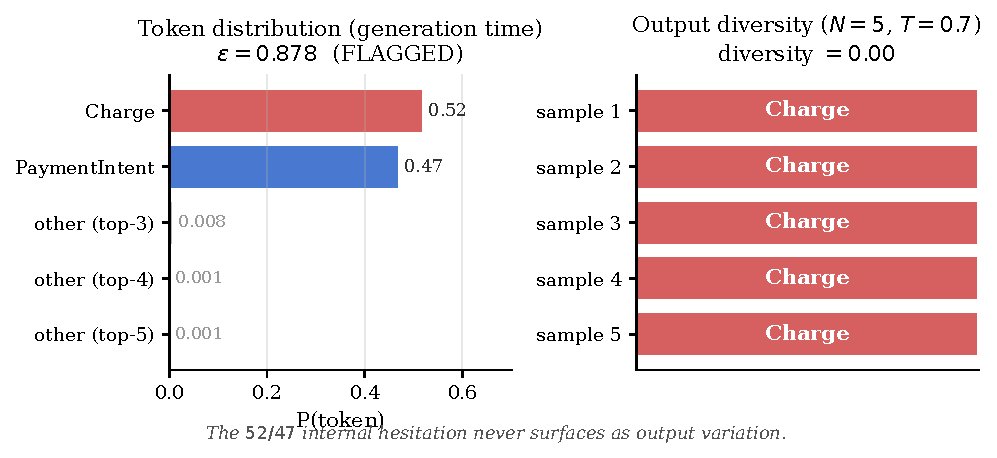
\includegraphics[width=0.85\textwidth]{figures/fig_intra_inter.pdf}
\caption{The intra/inter distinction made concrete on Stripe
Scenario A (GPT-4o). Left: the token distribution at the method-%
selector token shows a near-tie ($P(\texttt{Charge}) = 0.52$,
$P(\texttt{PaymentIntent}) = 0.47$), giving $\eps = 0.878$ at that
token. Right: five independent samples at $T=0.7$ all emit
\texttt{Charge} (diversity $= 0.00$). Multi-sample can only observe
the right panel; the left panel is what \eps reads. The $52/47$
internal hesitation never surfaces as output variation.}
\label{fig:intra-inter}
\end{figure}

Figure~\ref{fig:intra-inter} is the empirical proof of the intra/%
inter distinction, not a theoretical assertion. GPT-4o with $\eps =
0.878$ on Stripe chose \texttt{Charge} unanimously across all five
samples. A stronger multi-sample check would not recover the signal:
there is no output variation for a semantic-equivalence test or
symbolic executor to disagree about. Our multi-sample measurement
is output-level (which API was chosen); stronger equivalence
checks~\cite{sharma2025multisample} that compare code behaviour up
to semantic equivalence would help on Type 3 false positives, where
two semantically equivalent implementations are wrongly counted as
disagreement, but they cannot recover intra-generational API-choice
uncertainty that produces unanimous output.

UQLM~\cite{uqlm2024} is the closest published off-the-shelf tool in
this family; its \texttt{BlackBoxUQ} method samples each prompt
$5$ times and scores semantic disagreement via a DeBERTa NLI model.
On our benchmark it detects $5\%$ of \textsc{high}-risk prompts at
$0\%$ \textsc{low} false-positive rate --- a result driven by the
same structural limit: the model is behaviourally consistent even
when internally uncertain.

\subsection{Static analysis}
\label{subsec:static-cov}

Static analysis is complementary to \eps and is treated in
\S\ref{subsec:related-static}. The method requires only top-$k$
log-probabilities --- no model-internal access --- available via
OpenAI's \texttt{logprobs} parameter, DeepSeek via Together AI, and
vLLM for open-source models. Anthropic's API does not currently
expose per-token log-probabilities.

\subsection{Summary}
\label{subsec:comp-summary}

\begin{figure}[H]
\centering
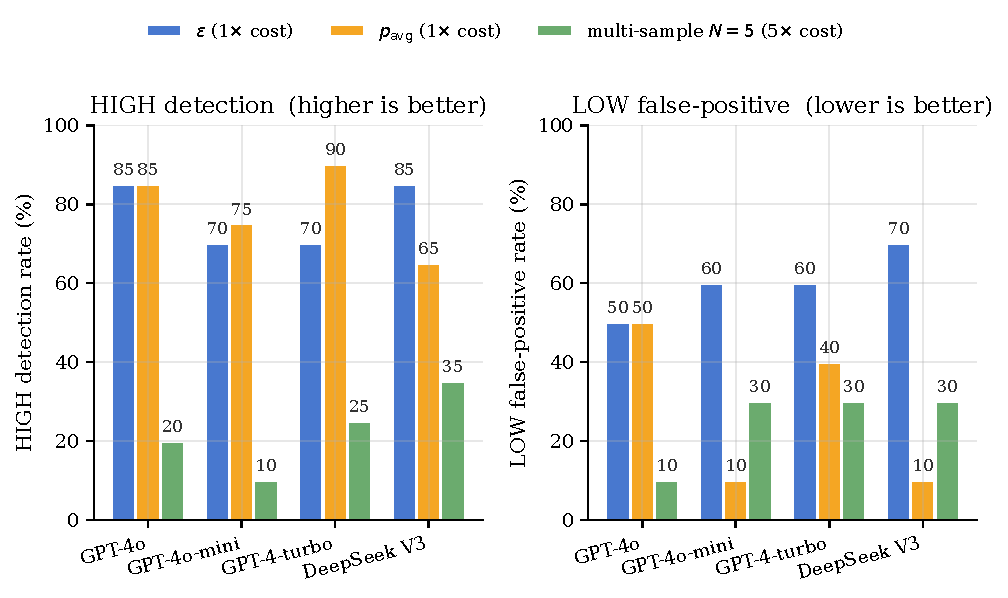
\includegraphics[width=\textwidth]{figures/fig_comparison.pdf}
\caption{Three-method comparison across four models. Left:
\textsc{high} detection rate (higher is better). Right: \textsc{low}
false-positive rate (lower is better). \eps and \papg operate at
$1\times$ API cost; multi-sample at $N=5$ costs $5\times$. \papg is
competitive with \eps on raw function-level detection; multi-sample
is structurally blind to intra-generational uncertainty.}
\label{fig:comparison}
\end{figure}

Through the full review loop (\S\ref{subsec:review-loop}), the
token-attribution gap becomes a precision gap: \eps achieves $94\%$
end-to-end precision; \papg-routed review, without token
localization, achieves $50.5\%$ on the same infrastructure
(Table~\ref{tab:pavg-endtoend}).
